% Apresentação de seminário - baseada em slide_template/main.tex
% Conteúdo derivado do artigo final (entrega2/main.tex)

\documentclass{beamer}

\usepackage[brazilian]{babel}
\usepackage[utf8]{inputenc}
\usepackage[T1]{fontenc}

\mode<presentation>
{
  \usetheme{default}
  \usecolortheme{default}
  \usefonttheme{default}
  \setbeamertemplate{caption}[numbered]
  \setbeamertemplate{navigation symbols}{}
}

\usepackage{graphicx}
\usepackage{booktabs}
\usepackage{amsmath, amssymb}
\usepackage{hyperref}

\usepackage[backend=biber]{biblatex}
\addbibresource{ref.bib}

\title[Rede pública x privada]{Distinção entre as áreas dos cursos de graduação ofertados pelas redes pública e privada no Brasil}
\author{Nathália Nunes \and João Gabriel \and Rafael Jordane}
\institute{Departamento de Estatística -- UFES \\ Disciplina: Dados Categóricos}
\date{\today}

\begin{document}

\begin{frame}
  \titlepage
\end{frame}

\begin{frame}{Roteiro}
  \tableofcontents
\end{frame}

% ===========================================================================
\section{Introdução}

\begin{frame}{Pergunta de pesquisa}
  \begin{block}{Objetivo}
    Investigar se há distinção clara entre os cursos de graduação ofertados pela rede \textbf{pública} e pela rede \textbf{privada} no Brasil.
  \end{block}
  \begin{itemize}
    \item A distinção pode se dar em mais de um eixo: além da \textbf{área}, examinamos o \textbf{grau acadêmico} e a \textbf{modalidade de ensino}.
    \item Entre 2014 e 2024, a matrícula na educação superior cresceu 30,5\%.
    \item Em 2024 são 45.776 cursos de graduação, das mais diversas áreas.
  \end{itemize}
\end{frame}

% ===========================================================================
\section{Dados}

\begin{frame}{Base de dados}
  \textbf{Censo da Educação Superior 2024 (INEP)}, Cadastro de Cursos.
  \begin{itemize}
    \item 720.349 cursos registrados, descritos por 223 variáveis.
    \item Filtro: apenas cursos de graduação (bacharelado, licenciatura, tecnólogo).
    \item Variáveis analisadas: rede, área geral (CINE), grau acadêmico, modalidade, região.
  \end{itemize}
  \begin{block}{Composição por rede}
    700.198 cursos (\textbf{97,2\%}) na rede privada; 20.151 (\textbf{2,8\%}) na pública.
  \end{block}
\end{frame}

% ===========================================================================
\section{Análise exploratória}

\begin{frame}{Perfil de áreas por rede}
  \begin{columns}
    \column{.5\textwidth}
    \textbf{Mais na rede pública}
    \begin{itemize}
      \item Educação ($+$24,0 p.p.)
      \item Engenharias ($+$3,9)
      \item Agricultura/Veterinária ($+$2,4)
    \end{itemize}
    \column{.5\textwidth}
    \textbf{Mais na rede privada}
    \begin{itemize}
      \item Negócios/Direito ($-$15,0 p.p.)
      \item Saúde ($-$6,8)
      \item Serviços ($-$5,7)
    \end{itemize}
  \end{columns}
  \vspace{1em}
  Curso típico: \textit{Negócios} na privada (29,6\%), \textit{Educação} na pública (43,6\%).
\end{frame}

\begin{frame}{Modalidade: o contraste mais forte}
  \begin{figure}
    \centering
    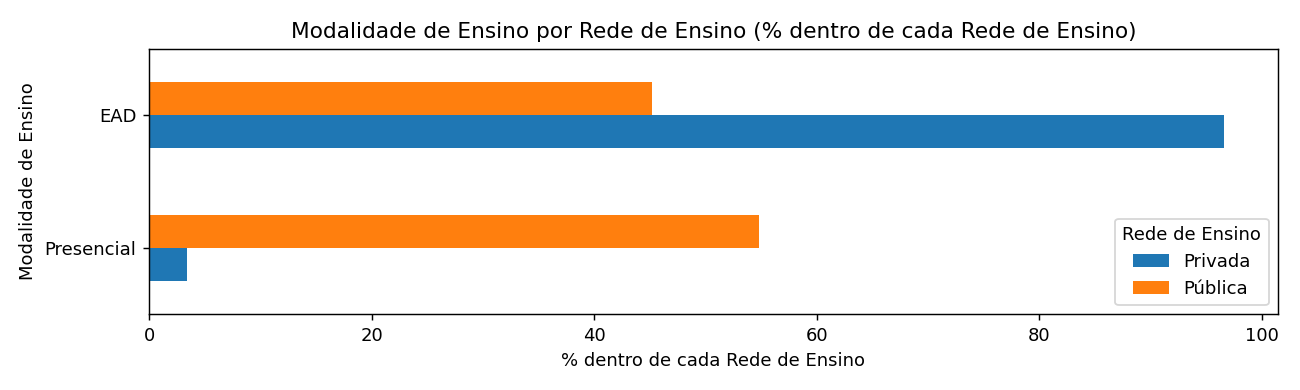
\includegraphics[width=.6\textwidth]{descritiva_plots/bi_TP_MODALIDADE_ENSINO_por_rede.png}
    \caption{Modalidade de ensino dentro de cada rede.}
  \end{figure}
  96,6\% da oferta privada é EAD, contra 45,2\% na pública.
\end{frame}

% ===========================================================================
\section{Metodologia}

\begin{frame}{Três métodos complementares}
  \begin{enumerate}
    \item \textbf{Qui-quadrado + V de Cramér + resíduos.} Mede a associação entre a rede e cada característica, uma de cada vez.
    \item \textbf{Regressão logística.} Estima a chance de um curso ser público controlando área, grau, modalidade e região ao mesmo tempo, com interação grau$\times$modalidade.
    \item \textbf{Modelo log-linear.} Trata rede, grau e modalidade sem eleger resposta; testa a interação tripla.
  \end{enumerate}
  \begin{block}{Por que três?}
    A análise vai ficando mais exigente: da associação bruta ao efeito ajustado e à associação simétrica de três vias.
  \end{block}
\end{frame}

\begin{frame}{Fórmulas centrais}
  \textbf{Qui-quadrado e V de Cramér}
  \[
    \chi^2 = \sum_{i,j} \frac{(n_{ij}-e_{ij})^2}{e_{ij}},
    \qquad
    V = \sqrt{\frac{\chi^2}{n\,(\min(I,R)-1)}}
  \]
  \textbf{Regressão logística (razão de chances)}
  \[
    \log\!\left(\frac{\pi(x)}{1-\pi(x)}\right) = \beta_0 + \sum_j \beta_j x_j,
    \qquad
    \text{OR}_j = e^{\beta_j}
  \]
  \textbf{Log-linear (modelo saturado de 3 vias)}
  \[
    \log(\mu_{ijk}) = \lambda + \lambda_i^{R} + \lambda_j^{G} + \lambda_k^{M} + \lambda_{ij}^{RG} + \lambda_{ik}^{RM} + \lambda_{jk}^{GM} + \lambda_{ijk}^{RGM}
  \]
\end{frame}

% ===========================================================================
\section{Resultados}

\begin{frame}{Método 1: força da associação}
  \begin{table}
    \centering
    \small
    \begin{tabular}{lrr}
      \toprule
      Cruzamento & $\chi^2$ (gl) & V de Cramér \\
      \midrule
      Rede $\times$ Área      & 11.846,4 (10) & 0,128 \\
      Rede $\times$ Grau      & 12.595,1 (2)  & 0,132 \\
      Rede $\times$ Modalidade & 112.638,1 (1) & \textbf{0,395} \\
      \bottomrule
    \end{tabular}
  \end{table}
  Todas com $p<2{,}2\times10^{-16}$. Na escala (0,1 fraca / 0,3 média / 0,5 forte), só a \textbf{modalidade} chega ao patamar médio a forte.
\end{frame}

\begin{frame}{Método 1: onde a associação se concentra}
  Resíduos padronizados de Pearson (referência: $|r|>2$):
  \begin{itemize}
    \item Pública $\times$ Educação: \textbf{$+$83,57} (excesso forte).
    \item Pública $\times$ Negócios: $-$46,19 (déficit forte).
    \item Pública $\times$ Tecnológico: $-$99,43.
  \end{itemize}
  \vspace{.5em}
  O resíduo mede quantos desvios-padrão a célula está acima ou abaixo do esperado sob independência.
\end{frame}

\begin{frame}{Método 2: razões de chance (evento = pública)}
  \begin{table}
    \centering
    \small
    \begin{tabular}{lrc}
      \toprule
      Termo & OR & IC 95\% \\
      \midrule
      \textbf{modalidadeEAD}   & \textbf{0,033} & [0,031; 0,034] \\
      Ciências nat./mat./est.  & 2,759 & [2,49; 3,06] \\
      Computação e TIC         & 2,064 & [1,93; 2,21] \\
      Saúde e bem-estar        & 0,329 & [0,303; 0,356] \\
      regiaoSul                & 0,611 & [0,582; 0,642] \\
      \bottomrule
    \end{tabular}
  \end{table}
  Pseudo-$R^2$ de McFadden $=0{,}324$. A EAD é o efeito mais extremo: um curso presencial tem cerca de 30 vezes mais chance de ser público que um a distância.
\end{frame}

\begin{frame}{Método 2: o efeito da EAD depende do grau}
  Efeito líquido da EAD (principal $\times$ interação):
  \begin{table}
    \centering
    \begin{tabular}{lrl}
      \toprule
      Grau & OR da EAD & Leitura \\
      \midrule
      Bacharelado (ref.) & 0,033 & presencial $\approx$ 30$\times$ \\
      Licenciatura & $\approx$ 0,023 & $\approx$ 44$\times$ \\
      Tecnológico  & $\approx$ 0,010 & $\approx$ 96$\times$ \\
      \bottomrule
    \end{tabular}
  \end{table}
  A EAD empurra a oferta para a rede privada nos três graus, com \textbf{mais força no tecnólogo}.
\end{frame}

\begin{frame}{Método 3: interação tripla}
  \begin{table}
    \centering
    \small
    \begin{tabular}{llrr}
      \toprule
      Grau & Modalidade & Pública & Privada \\
      \midrule
      Tecnológico & Presencial & 1.318 & 3.876 \\
      Tecnológico & EAD        & 1.153 & 332.227 \\
      \bottomrule
    \end{tabular}
  \end{table}
  \begin{itemize}
    \item Remover a interação tripla piora o ajuste: deviance $=654{,}13$ (2 gl, $p<2{,}2\times10^{-16}$).
    \item A associação rede$\times$modalidade muda conforme o grau: no tecnólogo, a pública se divide quase meio a meio, a privada é 98,8\% EAD.
  \end{itemize}
\end{frame}

% ===========================================================================
\section{Discussão}

\begin{frame}{A EAD virou terreno privado (não sempre foi)}
  \begin{itemize}
    \item Em 2002, a EAD ainda era majoritariamente \textbf{pública} (só 16\% privada) \parencite{pintoAcessoEducacaoSuperior2004}.
    \item Entre 2001 e 2006, as IES privadas de EAD cresceram 4.700\% contra 200\% na pública \parencite{segenreichExpansaoPrivatizacaoDiferenciacao2009}.
    \item Em 2024, 96,6\% da oferta privada é EAD.
  \end{itemize}
  \begin{block}{Tecnólogo + EAD}
    Mesmo pacote comercial, adotado pelas mesmas instituições no mesmo período: ciclo curto, sem pesquisa, escala e baixo custo \parencite{carvalhoMercantilizacaoEducacaoSuperior2013}.
  \end{block}
\end{frame}

\begin{frame}{Ressalvas e contraponto}
  \begin{itemize}
    \item \textbf{Colinearidade Educação $\approx$ Licenciatura} não é erro: quase toda licenciatura está na área Educação, área que o setor privado evita por baixo retorno.
    \item \textbf{Convergência curricular:} quando modalidade e área são fixadas, pública e privada se parecem \parencite{schonarth2016cstgq}. A distinção é de \emph{estratégia de oferta}, não de conteúdo.
    \item \textbf{Limites:} a base não separa privada lucrativa da não lucrativa; parte do efeito da rede pode ser do próprio grau.
  \end{itemize}
\end{frame}

% ===========================================================================
\section{Conclusão}

\begin{frame}{Conclusão}
  \begin{itemize}
    \item Existe distinção clara entre as redes, e o eixo mais forte é a \textbf{modalidade}, não a área.
    \item V de Cramér 0,395 (modalidade) contra 0,128 (área); OR da EAD 0,033.
    \item O contraste depende do grau: máximo no tecnólogo (interação tripla).
    \item A distinção é de estratégia de oferta. Serve de base para investigar os fatores por trás da oferta de cursos no Brasil.
  \end{itemize}
\end{frame}

% ===========================================================================
\section{Referências}

\begin{frame}[allowframebreaks]{Referências}
  \tiny
  \printbibliography[heading=none]
\end{frame}

\end{document}
